\section{Принцип индукции}

Пусть $P(n)$~--- некоторое утвержение, в котором как-то фигурирует натуральное число $n$. Пусть нам удалось доказать истинность $P(0)$, а так же следствие $P(n)\to P(S(n))$ для любого $n$, где функция $S(n)$ обозначает элемент, следующий за $n$. Используя это следствие, мы можем получить $P(0)\to P(1)$. Отсюда, опять же по тому же следствию $P(1)\to P(2)$. Затем $P(2)\to P(3)$. Продолжая так бесконечно долго, мы получаем, что утверждение истинно вообще для любого натурального $n$.

Приведенное рассуждение довольно неформально, фраза <<продолжая так бесконечно долго>> явно требует уточнения. Строгие рассуждения ниже довольно жесткие по содержанию, их можно пока пропустить до первого примера ниже, если у вас возникнут проблемы с пониманием. Более обстоятельно мы подобные рассуждения будем рассматривать в главе, посвящённой бесконечным множествам, и тогда у вас уже вопросов по этой теме не должно будет остаться.

Итак, давайте для примера вместо натуральных чисел рассмотрим множество $\mathbb{N}^2$, упорядоченное лексикографически. Напомню, что это значит, что мы рассматриваем пары натуральных чисел $(a, b)$, а для сравнения на больше и меньше используем тот же принцип, по которому упорядочены слова в словаре: вначале мы сравниваем первые числа, и только если они равны, то сравниваем вторые числа. Например:
$$(1, 2) < (10, 1)$$
$$(4, 4) > (4, 1)$$

Попробуем применить индукцию теперь к этому множеству. Из $P((0, 0))$ следует $P((0, 1))$, отсюда следует $P((0, 2))$, затем $P((0, 3)), P((0, 4))$ и так далее. Очевидно, что в этих рассуждениях мы никогда не достигнем даже значения $P((1, 0))$, поэтому метод индукции на таком множестве не работает.

Мы конечно это множество сконструировали специальным образом, но по большому счёту у нас нет никаких жестких гарантий, что в случае $\mathbb{N}$ индукция действительно достигнет каждого элемента. Вдруг всё же есть какой-то элемент $k\in \mathbb{N}$, который мы никогда не достигнем? Маловероятно, но нам надо быть уверенным, что подобного случаю $\mathbb{N}^2$ не произойдёт.

Предположим, действительно, что индукция не верна для $\mathbb{N}$ и непустое множество чисел, для которых утверждение $P(n)$ не выполняется, обозначим как
$$X = \{n\in\mathbb{N}|\neg P(n)\}$$
Это множество имеет минимальный элемент $m=\min X$, и поскольку это наименьшее число, для которого $P$ ложно, мы знаем, что $P(m-1)$ истинно. Однако отсюда и из импликации $P(n)\to P(S(n))$ следует истинность $m$, а это противоречие. Значит правда: для натуральных чисел индукция работает.

Метод индукции можно обобщить двумя способами. Во-первых, мы могли бы начинать наш отсчет не с P(0), а с произвольного элемента $P(k)$. На доказательство и общий принцип применения индукции это никак не повлияло бы, поэтому мы не будем рассматривать этот случай.

Второе обобщение индукции заключается в том, что вместо импликаии $P(n)\to P(S(n))$ мы могли бы рассматривать импликацию $(\forall m<n, P(m))\to P(n)$. Здесь мы в доказательстве опираемся не только на одно значение $n$, но на все значения, меньшие заданного, для которых уже доказана истинность $P(m)$. Справедливость такого принципа индукции доказывается аналогично: если бы существовало непустое множество чисел $X$, для которых утверждение неверно, мы могли бы взять минимальный элемент этого множества $m$, а отсюда мы сразу же приходим к противоречию как и в первом случае.

Первоначальный подход называется \term{слабой индукцией}, последний подход называется \term{сильной индукцией}. Если рассматривать только натуральные числа, то разница между двумя индукциями невелика. Слабая индукция следует из сильной при замене $\forall m<n P(m)$ на $P(n-1)$, сильная индукция может получиться из слабой, если ввести множества
$$A_i = \{0, 1, 2, \ldots, i\}$$
и доказывать, используя слабую индукцию, утверждение
$$P'(n) = \forall x \in A_n, P(x)$$
вместо первоначального $P(n)$. То есть эти подходы эквивалентны.

Тем не менее, сильная индукция может быть легко обобщена на довольно широкий класс множеств: если внимательно вглядеться в доказательство сильной индукции, то единственное, что мы требуем от множества, на котором формулируем принцип индукции, это чтобы любое его подмножество $X$ имело минимальный элемент. В первом параграфе мы называли такие множества фундированными, и теперь понятно, почему они заслуживают отдельного определения: такие множества (и только такие, см. упражнение ниже) допускают применять к себе принцип индукции.

Пока что мы не будем всерьез заниматься индукцией на произвольных фундированных множествах, вернувшись к ним в главе, посвященной бесконечным множествам, но в качестве необязательного попробуйте доказать следующее

\begin{exercise}
Пусть на множестве $X$ работает принцип сильной индукции. Докажите, что это множество фундированное.
\end{exercise}

Всё, что мы до сих пор говорили, относилось только к аксиоматике Фреге-Рассела, однако из сформулированных нами аксиом Пеано принцип индукции вывести невозможно. Напомню, что мы определили аксиомы Пеано как некоторое множество с заданной на нём инъективной функцией $S$, для который 0 не имеет обратного элемента. Дополнительно мы ввели определение сложения, умножения и возведения в степень (см.\S3.1). Обозначим этот набор аксиом как $\mathbb{P}^-$.

Если внимательно посмотреть на доказательство слабой индукции, то можно заметить, что мы по элементу $m=\min X$ для построения противоречия искали \term{предыдущий элемент} $m-1$. То есть мы неявно предполагали существование функции
\begin{align*}
S: & \mathbb{N}\{0\} \to \mathbb{N}\\
    & n \mapsto n-1
\end{align*}
Для аксиом Фреге-Рассела определить её легко:
$S^{-1}(n) = \{k \in n | S(k) \in n\}$
Эта формула станет понятной, если вы вспомните, что
$$n = \{0, 1, 2, \ldots, (n-1)\}$$
А вот из $\mathbb{P}^-$ определить такую функцию уже невозможно. Почему? Ответ здесь кроется в том, и $\mathbb{N}$ в терминах Фреге-Рассела, и введённое выше множество $\mathbb{N}^2$ оба являются моделями для $\mathbb{P}^-$. В последнем случае элемент $(1, 0)$ предыдущего элемента не имеет. Ну и плюс к этому, поскольку в первом случае слабая индукция работает, а во втором не работает, то это значит, что принцип слабой индукции из $\mathbb{P}^-$ вовсе не выводим никак (см.\S1.5).

Итак сформулированные нами до сих пор аксиомы Пеано $\mathbb{P}^-$ не полноценны, пока мы не добавим к ним аксиому индукции:
$$(P(0)\land(\forall n (P(n)\to P(S(n)))) \to \forall m, P(m)$$
Вот теперь определение аксиоматики Пеано нами завершено и с этой дополнительной аксиомой какие-то <<нестандартные модели>> арифметики хоть и возможны, но строятся уже не так просто и мы их рассматривать не будем. Простейшие примеры типа $\mathbb{N}^2$ теперь не проходят, т.к. прицнип слабой индукции накладывает очень серьезные ограничения на модель. Я замечу, что вместо аксиомы индукции можно было бы потребовать выполнения каких-то других аксиом, например потребовать, чтобы функция $S|_{\mathbb{N}\backslash\{0\}}$ была обратима, однако такие варианты аксиом видимо менее интуитивно понятны, поэтому редко формулируются в таком виде.

Перейдём от теории к практике и рассмотрим примеры применения принципа индукции.

\begin{example}
Докажем закон Де Моргана для произвольного конечного набора множеств:
\begin{equation}\label{ni:1}
\left(\bigcup_{i=0}^n A_i\right)^C = \bigcap_{i=0}^n A_i^C
\end{equation}
\end{example}

Формула \eqref{ni:1} будет выступать у нас в роли доказываемого предложения $P(n)$. Мы будем начинать отсчет индукции не с $P(0)$, а с $P(2)$, поскольку это первый нетривиальный случай:
\begin{equation}\label{ni:2}
(A\cup B)^C = A^C \cap B^C
\end{equation}
Это мы уже доказывали в параграфе \S~2.1. Теперь докажем импликацию $P(n)\to P(n + 1)$. Запись $S(n)$ будем использовать для обозначения исходного выражения.
$$S(n+1) = \left( \bigcup_{i=0}^{n+1} A_i \right)^C = \left( \left( \bigcup_{i=0}^n A_i\right) \bigcup A_{n+1}\right)^C$$
К этому выражению применимо тождество \eqref{ni:2}, из которого получаем
$$S(n+1) = \left( \bigcup_{i=0}^n A_i\right)^C \bigcap A_{n+1}^C$$
Однако мы предполагаем, что $P(n)$ истинно, поэтому к выражению слева мы можем легко применить \eqref{ni:1}:
$$S(n+1) = \left(\bigcup_{i=0}^n A_i^C\right) \bigcap A_{n+1}^C = \bigcup_{i=0}^{n+1} A_i^C$$
А это ровно то, что требовалось доказать. Это же самое доказательство работает и для пересечения множеств и для логических операций.

\begin{example}
Докажите, что в выражении
$$a_0 a_1 a_2 \ldots a_n$$
где $a_i$ натуральные числа, не важно как расставлять скобки.
\end{example}

Уветрждение кажется очевидным, но на самом деле это не так. Пусть есть четыре числа 100, 234, 135 и 77. Мы тут утверждаем, например, что
$$(100\cdot 234)\cdot (135 \cdot77) = 23400 \cdot 10395 = 3159000 \cdot 77 = ((100\cdot 234)\cdot 135) \cdot77$$
То что это действительно так все знают, это кажется очевидным, так как мы привыкли к такому с детства, хотя в школе этого и не доказывали: к этому приучали. Но вообще-то это надо доказывать, так как если просто смотреть на конкретные числа, данные равенства выглядят уже не слишком убедительно сами по себе.

Прежде чем двигаться дальше, я советую читателю попробовать доказать утверждение примера самостоятельно~--- это совершенно не сложно. Только когда попытаетесь порассуждать сами, читайте дальше.

Простейший нетривиальный случай это $P(3)$~--- его мы доказали в~\S3.1, это обычный закон ассоциативности. Далее воспользуемся сильной индукцией: предположим что верно $\forall m<n, P(m)$ и докажем отсюда $P(n)$. Пусть изначально скобки расставлены следующим образом:
$$(a_0\ldots a_k)(a_{k+1}\ldots a_n)$$
Это означает, что сначала в некотором порядке отдельно будут перемножены группы чисел $a_0\ldots a_k$ и $a_{k+1}\ldots a_n$, а затем будут перемножены результаты. Внутри этих групп числа могут перемножаться в любом порядке в силу предположения индукции. Для того, чтобы доказать возможность произвольной расстановки скобок, нам надо показать, что это выражение эквиваленно
$$(a_0\ldots a_m)(a_{m+1}\ldots a_n)$$
где $m$~--- некий произвольный номер. Будем считать для определённости, что $m>k$, случай $m<k$ доказывается аналогично. Имеем:
$$(a_0\ldots a_k)((a_{k+1}\ldots a_m)(a_{m+1}\ldots a_n))$$
По закону ассоциативности это можно записать как
\begin{align*}
((a_0\ldots a_k)(a_{k+1}\ldots a_m))(a_{m+1}\ldots a_n)\\
= (a_0\ldots  a_m)(a_{m+1}\ldots a_n)
\end{align*}
Теперь мы можем вначале умножить группу чисел $a_0\ldots a_m$, затем группу чисел $a_{m+1}\ldots a_n$, причем обе группы могут умножаться в произвольном порядке, $m$ мы так же выбрали произвольно. А это ровно то, что требовалось доказать.

Полностью аналогичное доказательство возможно и для любых прочих операций, обладающих свойством ассоциативности: логических операций, арифметического сложения, операций над множествами и т.д.

В действительности многие доказательства прошлых параграфов были весьма урезанны в силу того, что мы не доказывали индуктивный шаг, полагая это чем-то очевидным. Это, конечно, совершенно не так, и для строгости надо было доказывать это по индукции. Вот несколько примеров:

\begin{exercise}
Объясните чем было плохо доказательство
$$m^n = \underbrace{m\cdot m \cdot \ldots \cdot m}_n$$
и докажите это корректно.
\end{exercise}

\begin{exercise}
Объясните где была дырка в доказательстве основной теоремы арифметики, и заткните эту дырку.
\end{exercise}

\begin{exercise}
Докажите, что декартово произведение конечных множеств~--- конечно.
\end{exercise}

\begin{exercise}
Докажите по индукии равенство $ab=ba$ исходя из аксиом Пеано. Это сложное доказательство и вначале вам придется доказать кучу промежуточных фактов о сложении и умножение, и всё это тоже делается по индукции~--- я не рассчитываю, что вы самостоятельно доведёте работу до конца, но по крайней мере попытка будет не лишней.
\end{exercise}

И так далее. Если доказывать основы арифметики строго и из аксиом Пеано, не опуская скучные детали, то там в каждой теореме индукция будет применяться по три-четыре раза минимум. Этим редко кто занимается, не стали этим заниматься и мы.

Всё сказанное до сих пор относилось больше к теории и по большому счёту мы доказывали то, что уже знали. Перейдём теперь к более приземленным примерам.

\begin{example}Обозначим
$$S(n) = 1 + 2 +3 \ldots + n$$
и
$$S'(n) = {n(n+1)\over 2}$$
Доказываемое утверждение $P$ будет состоять в том, что
$$S(n) = S'(n)$$
то есть что две приведенные две формулы эквивалентны.
\end{example}

Равенство $S(0) = S'(0)$ довольно очевидно, нам теперь надо доказать импликацию $P(n)\to P(n + 1)$, то есть доказать, что если эти формулы совпадают для произвольного $n$, то они будут совпадать и для $n + 1$. В соответствии с определением, для любого $n$
$$S(n + 1) = 1 + 2 + \ldots + n + (n + 1)$$
Из предположения о том, что утверждение верно для $n$, мы первые $n$ слагаемых можем переписать, используя формулу для $S'$:
\begin{align*}
S(n + 1) &= {n(n + 1)\over 2} + (n + 1)\\
	&= {n^2 + n\over 2} + {2n + 2\over 2} \\
	&= {n^ 2 + 3n + 2 \over 2} \\
	&= {(n + 1)(n + 2)\over 2} \\
	&= {S'(n + 1)}
\end{align*}

Всё! Мы доказали, что из равенства $S(n)=S'(n)$ следует так же равенство $S(n+1)=S'(n+1)$, а это всё что требуется: теперь принцип индукции гарантирует нам, что действительно для любого $n$ эти формулы совпадают.

Принцип индукции чрезвычайно силён: подаляющее большинство теорем, в которых как-то фигурируют произвольные натуральные числа, могут быть доказаны таким образом, причем во многих случаях доказательство оказывается не сложным. С другой стороны этот метод обладает и явным недостатком: он позволяет нам доказать утверждение, которое нам уже известно, но не даёт никакого способа это утверждение вывести, не зная ответа. Например, если бы задача изначально состояла не в том, чтобы доказать равенство двух формул, а в том, чтобы получить краткое выражение для $S(n)$, метод индукции нам уже почти никак не помог бы.

Часто о решении можно догадаться. Например, если записать первые значения $S(n)$
$$0, 1, 3, 6, 10, 15, 21, 28, 36, \ldots$$
то некоторые смогут увидеть закономерность $S'$. По крайней мере так пишут в учебниках, что догадаться можно, а в жизни я людей, которые легко улавливают такие закономерности, видел очень мало. Но предположим, что догадаться можно.

Чаще формулу можно подобрать. Для $S(n)$ мы могли бы предположить, что формула имеет вид
$S(n) = {an^2 + bn + c\over d}$
где $a, b, c, d$~--- некоторые неизвестные нам числа. Затем, вычислив явно значения $S(0), S(1), S(2), S(3)$ можно убедиться в том, что единственными вариантом, который работает, является набор значений
$$a=1, b=3, c=2, d=2$$
Эти значения приводят к формуле $S'(n)$, но это пока не является доказательством, поскольку мы проверили эту формулу лишь на четырёх значениях $n$, но по крайней мере нам уже есть к чему приложить принцип индукции.

Этот подход может показаться так же сложным и надуманным, но на самом деле он довольно прост. Если нарисовать значения $S(n)$ на графике, то их расположение будет очень сильно похоже на параболу, которую тут же распознает любой смышленный школьник, а формула с неизвестными, которую я привёл выше~--- это как раз формула параболы в общем виде. Мы пока не рассматривали графики функций, поэтому такое рассуждение может показаться сложным или необычным, но через какое-то время вы научитесь довольно быстро искать такие решения самостоятельно.

Тем не менее даже если мы формулу каким-то образом подобрали, а потом доказали её, нам хочется её еще и понять. Да, мы знаем, что $S(n)=S'(n)$, но с какой стати? Эти две формулы совершенно не похожи друг на друга и их взаимосвязь совершенно не ясна. Это главная проблема принципа индукции: он позволяет доказать очень многое, но он совершенно не проясняет ситуацию.

Попробуем вывести краткую формулу для $S(n)$, зайдя с другого угла. Для этого вначале расположим красные квадраты в ряды один под другим (рис.3.8). В первом ряду у нас будет один квадрат, во втором два, в третьем три и так далее. Наша задача~--- подсчитать сколько всего получается квадратов, если мы располагаем таким образом квадраты в $n$ строчках. Как видно из картинки, эти квадраты образуют некое подобие треугольника, поэтому такие числа называются \term{треугольными}.

\begin{figure}[h]
\centering
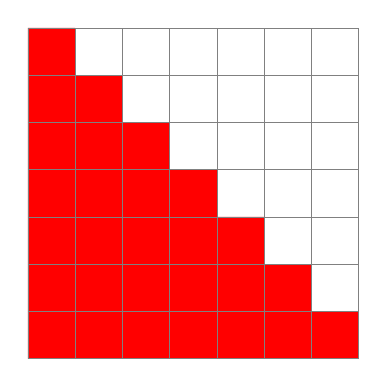
\begin{tikzpicture}
  \fill[red] (0, 0) -- (4.2cm, 0) -- (4.2cm, .6cm) -- (3.6cm, .6cm) -- (3.6cm, 1.2cm) -- (3cm, 1.2cm) -- (3cm, 1.8cm) -- (2.4cm, 1.8cm) -- (2.4cm, 2.4cm) -- (1.8cm, 2.4cm) -- (1.8cm, 3cm) -- (1.2cm, 3cm) -- (1.2cm, 3.6cm) -- (.6cm, 3.6cm) -- (.6cm, 4.2cm) -- (0, 4.2cm) -- cycle;
  \draw[step=.6cm,gray,very thin] (0, 0) grid (4.2cm,4.2cm);
\end{tikzpicture}
\caption{Треугольные числа}
\end{figure}

Помимо квадратов я изобразил сетку, одна ячейка которой по размеру равняется величине квадрата, а строк и колонок в ней $n$ штук. Всего клеток, таким образом, имеется $n^2$. Из всех этих клеток красные клетки~--- это те, что лежат на диагонали (их $n$ штук), а так же половина от оставшихся клеток. Итого, мы получаем
$$S(n) = {n^2 - n\over 2} + n = {n^2 - n + 2n \over 2} = {n(n+1)\over 2}$$
Без каких-либо хитрых умоизысканий мы получили ту же самую формулу, причем теперь нам вполне понятно откуда она взялась и что означает.

В этом примере метод индукции оказался одновременно и сложнее и менее информативным~--- последний подход показал нам общую идею откуда такая формула берется, а не просто дал доказательство. Часто именно так и происходит, поэтому мы чаще всего будем избегать формальных выкладок по индукции и приводить по возможности методы, которые как-то раскрывают суть теоремы, а не просто доказывать что-то лишь бы доказать.

Тем не менее, последнее доказательство с клетками в строгом смысле доказательством не является. Как мы уже говорили в первой главе, строгое доказательство~--- это последовательность предложений, выводимых из аксиом с использованием четко определенного набора правил. Доказательство с клетками далеко от такого принципа: мы не определили никаких геометрических понятий, мы никак не определили по какому вообще критерию мы отождествляем клетки с числами, мы никак даже не определяем понятие положения клеток в пространстве. Безусловно, доказательство выглядит убедительным (и, пролив много пота и крови, его можно сделать абсолютно строгим) и у большинства людей оно справедливо не будет вызывать сомнений. Однако формально этого не достаточно: многие учителя (не самые умные представители) в университетах такие доказательства не примут, так же подобное доказательство не признают многие авторы учебников, эти люди всюду доказывают любую мелочь по индукции. Я считаю это неправильным (правда, я и образования не получил), поэтому мы будем по возможности избирать не всегда самый формально корректный, но по возможности самый содержательный метод доказательства.

\begin{exercise}
Докажите, что
$$1^2 + 2^2 +3^2 \ldots + n^2 = {n(n+1)(2n+1)\over 6}$$
\end{exercise}

\begin{exercise}
Прошлое упражнение задаёт формулу для так называемых \term{пирадиальных квадратичных} чисел. Их можно рассматривать как число блоков из котороых состоит кирпичная пирамида с четырёхугольным основанием. Придумайте формулу для числа кирпичей в случае, если бы основанием пирамиды был треугольник. Такие числа называются \term{тэтраэдрическими пирамидальными}.
\end{exercise}

\begin{exercise}
Докажите, что
$$1^3 + 2^3 +3^3 \ldots + n^3 = \left({n(n+1)\over 2}\right)^2$$
\end{exercise}

Скорее всего в этих упражнениях вам придется воспользоваться методом индукции и это не даст вам никакой догадки о том, почему эти формулы работают. Далее мы немного углубимся в природу этих формул и выведем общую закономерность, хотя даже это не сильно поможет нам с интуитивным пониманием~--- хоть они и станут понятнее, красивой интерпретации как с треугольными числами мы получить всё равно не сможем (она в принципе есть в многомерных пространствах, но это не делает вещи проще). Иногда и такое бывает.

\begin{example}
Числами Ферма называются числа
$$F_n = 2^{2^n} + 1$$
Если записать первые числа Ферма
$$3, 5, 17, 257, 65537, 4294967297$$
то можно увидеть закономерность
\begin{equation}\label{ni:3}
F_n = \prod_{i=0}^{n-1}F_i + 2
\end{equation}
\end{example}

Давайте докажем это по индукции. Как обычно предположим, что для формула верна для $F_n$ и докажем из этого её правильность для $F_{n+1}$, переписав правда это несколько в другой форме:
\begin{align*}
\prod_{i=0}^n F_i &= (\prod_{i=0}^{n-1} F_i) F_n = (F_{n - 1} - 2) F_n \\
	&= (2^{2^n} - 1) (2^{2^n} + 1) = 2^{2\cdot 2^n} - 1 \\
	&= 2^{2^{n+1}} - 1 = F_{n+1} - 2
\end{align*}

Что и требовалось доказать.

Числа Ферма имеют интересную историю. Ферма их придумал в 1640-ом году и выдвинул гипотезу, что все такие числа простые. Действительно: они на вид походи на простые. Однако в 1732 годы Леонард Эйлер сумел разложить четвертое число Ферма на множители:
$$F_5 = 4294967297 = 641 \cdot 6700417$$
На это потребовалось почти сто лет! Интересно, что до сих пор не известно существует ли хоть одно простое число Ферма большее $F_4$~--- до сих пор все числа Ферма оказывались составными, однако исследована лишь малая доля таких чисел. Например, доказано, что число $F_{20}$ не является простым, хотя сами его множители не изветны~--- это уже слишком большое число, чтобы его можно было найти хотя бы один его делитель.

Тем не менее числа Ферма с простыми числами явно связаны. Например, легко видеть из~\eqref{ni:3} и теоремы~3.14, что число $F_n$ не имеет общих множителей с числами $F_i$ при $i<n$. Другими словами это значит, что все числа Ферма взаимопросты. Отсюда в частности следует, что простых чисел бесконечно много: если бы их было конечное число, мы не могли бы иметь бесконечную последовательность взаимопростых чисел. Мы таким образом еще раз доказали теорему Евклида, но уже другим способом.

Рассмотрим теперь два классических примера неправильного применения индукции.

\begin{example}
Докажем, что все лошади одного цвета. Пусть $A_n$~--- множество из $n$ лошадей, индукцию будем проводить по $n$ относительно уствержения <<в любом множестве $A_n$ все лошади имеют одинаковый цвет>>. Для $A_1$ утвержедение очевидно. Предположим, что утверждение верно для $A_m$ при $m<n$, и в этом предположении докажем верность утверждения для $A_n$. Разобьём множество $A_n$ на непустые непересекающиеся подмножества $B\cup B \cup\{x\}$, где $x$~--- одна отдельно взятая лошадь. По предположению индукции во множествах $B\cup\{x\}$ все лошади имеют один цвет, а то же самое касается множества $C\cup\{x\}$. Поскольку в обапоследних множества входит один и тот же $x$, то цвет лошадей в обоих множествах совпадает. Отсюда по индукции следует, что для любого $A_n$ цвет лошадей в этом множестве будет одинаковым. Что и требовалось доказать.
\end{example}

Рассуждение, очевидно, ошибочно, но обычно в подобных доказательствах не сразу понятно в чем ошибка. Проблема кроется в том, что когда мы предположили верность утверждения для $m<n$ мы забили о том, что $n$ в том числе может быть равно, двойке, а если это так, то множество $A_2$ невозможно разбить на непустые непересекающиеся $B\cup C\cup\{x\}$. Поэтому наше доказательство некорректно, но поучительно: всегда надо держать в голове крайние случаи, так как они часто приводят к проблемам.

\begin{exercise}
Докажем, что мы можем поднять любую гору песка. Будем проводить индукцию по количеству песчинок. Очевидно, что мы можем поднять одну песчинку. Но если предположить, что мы можем поднять $n$ песчинок, то и $n+1$ песчинку тоже поднять сможем, потому что каждая отдельная песчинка ничего почти не весит. А отсюда по индукции мы можем поднять вообще любое количетсво песчинок. Как считаете, почему это доказательство некорректно?
\end{exercise}
